\documentclass[12pt]{article}

\usepackage[utf8]{inputenc} 
%\usepackage[T1]{inputenc} 

\usepackage[french]{babel}
\usepackage{listings}

\usepackage{graphicx}
\usepackage[usenames]{color}
\usepackage{amsmath}
\usepackage{amssymb}
\usepackage{amsfonts}

\usepackage{framed}
\usepackage{enumerate}
%
\usepackage{tabularx}
\usepackage{mathrsfs}
\usepackage{tikz}
%\usepackage{calrsfs}
\usepackage{fontawesome}
% \usepackage{rotating}
\usepackage{adjustbox}
\usepackage{pifont}
\usepackage{textcomp}

%%%%%%%%%%%%%%%%%%%%%%%%%%%%%%%%%%%%
%%%%%%%%%%%%%%%%%%%%%%%%%%%%%%%%%%
\newcommand\bareme[1]{\makebox[0pt][r]{({\bf #1} pts)\hspace{0.8cm}}}

%%%%%%%%%%%%%%%%% Algorithmes %%%%%%%%%%%%%%%%%%%%%%%%%%%%
\usepackage{algorithm,setspace}
\usepackage{algpseudocode}

\algrenewcommand\algorithmicfunction{\textbf{fonction}}
\algrenewcommand\algorithmicend{\textbf{fin}}
\algrenewcommand\algorithmicdo{\textbf{faire}}
\algrenewcommand\algorithmicfor{\textbf{pour}}
\algrenewcommand\algorithmicif{\textbf{si}}
\algrenewcommand\algorithmicelse{\textbf{sinon}}
\algrenewcommand\algorithmicthen{\textbf{alors}}
\algrenewcommand\algorithmicreturn{\textbf{retourner}}
\algrenewcommand\algorithmicwhile{\textbf{tant que}}

\newcommand\com[1]{\Comment{\scriptsize\textcolor{red}{#1}\normalsize}}
%%%%%%%%%%%%%%%%%%%%%%%%%%%%%%%%%%%%%%%%%%%%%%%%%%%%%%%%%%



\newcommand{\red}{\textcolor{red}}   

\addtolength{\topmargin}{-0.8in}
\addtolength{\textheight}{1.2in} 
\addtolength{\oddsidemargin}{-50pt}
\addtolength{\textwidth}{100pt} %%%%
\addtolength{\parindent}{-\parindent}

\graphicspath{{./graphics/}}

\title{INF1132 Session Automne 2022\\Devoir 2\\}
\author{Professeurs : Sre\v{c}ko Brlek,  kelrB ok\v{c}erS} %Diego Maupomé}  
\date{}

\makeatletter
\renewcommand\contentsname{\center Pondérations}

%%%%%%%%%%%%%%%%%%%%%%%%%%%%%%%%%%

\begin{document}
\allowdisplaybreaks

\maketitle

\thispagestyle{empty}

%%%%%%%%%%%%%%%%%%%%%%%%%%%%%%%%%%

\hrule
\bigskip
Nom: NIARE YAYA
\bigskip
\hrule
\bigskip
Code permanent: NIAY84360305
\bigskip
\hrule
\bigskip
% Si s'applique, personne(s) avec qui vous avez collaboré (nom et groupe):\\
\bigskip
% \hrule


\begin{center}
\begin{tabular}{|c|c|c|c|c|c|}
\hline
1& 2  &  3 &  4 & 5 &\textbf{Total} \\
\hline
 &  &  & & &  \\
~~~~~~~/ $20$~ & ~~~~~~~/ $20$~  & ~~~~~~~/ $20$~& ~~~~~~~/ $20$~& ~~~~~~~/ $20$~ & ~~~~~~~~~~~~\textbf{/ $100$}~\\
&  &  &  & &\\
\hline
\end{tabular}
\end{center}

  \begin{framed}
	  \begin{footnotesize}
		  \centerline{\large\textbf{Directives}}
		  \begin{enumerate}
		    \item Le devoir doit être rédigé \textbf{individuellement} et remis \textbf{avant le \textcolor{red}{8 décembre 2022 avant midi}}.
		    \item \textbf{Aucun retard} n'est permis, car la solution sera mise en ligne après l'heure limite de remise.
		    
		    \item Votre document doit être {\textcolor{red}{\textbf{rédigé en \LaTeX{} }}}, à partir du modèle fourni incluant la page de couverture.
		    \item Vous devez remplir cette page comme page couverture pour vous identifier lors de la remise de votre devoir sinon votre travail \textbf{ne sera pas corrigé}.
		    \item Vous devez remettre sur Moodle \textcolor{red}{\textbf{un fichier compressé (.zip) contenant le pdf de votre devoir ET le code \LaTeX{} ayant servi à le générer.}} 
		    \item Pour que votre devoir soit corrigé, l'archive doit obligatoirement être nommée :\\ \textcolor{red}{\textbf{VOTRECODEPERMANENT\_INF1132\_DEVOIR2.zip}}. 
		    
		    \item À moins d'avis contraire, \textcolor{red}{vous devez \textbf{justifier} chacune de vos réponses}.
		    \item La démarche ainsi que l'utilisation correcte de la notation mathématique seront évaluées.
		  \end{enumerate}
	  \end{footnotesize}
  \end{framed}
  
  
\newpage

%%%%%%%%%%%%%%%%%%%%%%%
%
%   Question 1
%
%%%%%%%%%%%%%%%%%%%%%%%

%%%%%%%%%%%%%%%%%%%%%%%%
%
%   Question 1
%
%%%%%%%%%%%%%%%%%%%%%%%

\noindent
{\textsc{\underline{Question 1 sur les algorithmes et la complexit\'e (\textbf{20} points)}}} %
\\

Les parties A et B sont \underline{ind\'ependantes}.\\

\textbf{Partie A} (10 points)\\



Soit $a = (a_1, a_2, ..., a_n)$ une suite d'entiers naturels. Consid\'erons l'algorithme suivant



%        \begin{algorithm}
%         \setstretch{1}

\rule{0.8\textwidth}{0.4mm}
            \begin{algorithmic}[1]
                \Procedure{Mystere} {$T$ : Tableau d'entiers} 
                    \State $n \gets Longueur(T)$
                    \State $i \gets 0 $
                    \While{$ i < n-1$}
                       \State $p \gets i$
                        \For{$j \gets i+1,i+2,..., n-1$}
                           \If{$T[j] < T[p]$} {$p\gets j$}\EndIf
                        \EndFor
                        \State $t\gets T[p] ; T[p] \gets T[i] ; T[i] \gets t$
                        \State $i \gets i+1$
                    \EndWhile
                \EndProcedure
            \end{algorithmic}
\rule{0.8\textwidth}{0.4mm}
%        \end{algorithm}

        
\vspace{.25in}
\begin{enumerate}[1)]
\item \bareme{5}Faites une trace de l'ex\'ecution de l'algorithme {\tt Mystere} dans le cas de
la suite \bigskip

\centerline{{\large \tt T = (-3, 0, 10, -11, 0, 13, -9, 17).}}


\medskip
Plus pr\'ecis\'ement, vous devez donner les valeurs de {\tt i}, {\tt p} et 
{\tt T[0],T[1],T[2],...,T[7]}
apr\`es  chaque it\'eration de la boucle ext\'erieure {\bf tant que} 
(\`a la ligne 10).\\
\smallskip

\begin{framed}


{\large
\begin{center}
{\tt
\begin{tabular}{|r|r|r|r|r|r|r|r|r|r|} \hline
i&~p~&T[0]&T[1]&T[2]&T[3]&T[4]&T[5]&T[6]&T[7]\\  \hline
 & & -3& 0&10 &-11& 0& 13& -9&17\\  \hline
0 & 3& -11& 0& 10& -3& 0& 13& -9&17 \\  \hline
1 & 6& -11& -9& 10&  -3& 0& 13& 0&17 \\  \hline
2 & 3& -11& -9& -3&  10& 0& 13& 0&17 \\  \hline
3 & 4& -11& -9& -3& 0& 10& 13& 0&17  \\  \hline
4 & 6& -11& -9& -3&  0& 0& 10& 13&17 \\  \hline
5 & 6& -11& -9& -3&  0& 0& 10& 13&17 \\  \hline
6& 6& -11& -9& -3&  0& 0& 10& 13&17 \\  \hline
\end{tabular}}
\end{center}
}
\end{framed}
\vspace{.25in}
\item \bareme{2}
Que fait cet algorithme?
\begin{framed}
R\'EPONSE:
Cet algorithme permet de trier de dans l'ordre croissant le suite de nombre entier a = (a1, a2 , ... , an).

\end{framed}

\vspace{.25in}
\item \bareme{3}
Donnez un estim\'e avec la notation ${\cal O}$ du nombre de comparaisons effectu\'ees par cet algorithme en fonction de $n$. 


\begin{framed}
R\'EPONSE:
Je donne une notation ${\cal O}$ du nombre de comparaisons éffectuées en fonction de $n$ : \\
Soit $x$ le nombre de comparaison : \\
$x$ = $((n+(n-1))+(n+(n-3))+...+1)+n-1$ \\
$x$ = $n^2+(n-1)$ donc x est ${\cal O}(n^2)$ \\

\end{framed}

\item \bareme{5} {\bf Question Bonus}.
Donnez un exemple de tableau d'entiers pour le {\bf pire cas} et un exemple pour le {\bf meilleur cas} de l'algorithme {\tt Mystere} et donner dans chacun des cas le nombre de comparaisons effectu\'ees

\begin{framed}
R\'EPONSE:
Le pire ou le meilleur des cas dependent de la longueur du tableau.
Je donne un exemple de tableau d'entier  et nombre de comparaison éffectuée: \\
T = (7,0,32,-3,2,-17); n=6; \\
$x$ =$6^2+(6-1)$ \\
$x$ = $41$ donc il y'aura 41 comparaisons éfféctuées dans le pire ou le meilleur des cas. \\
\end{framed}

\end{enumerate}
%



\newpage
\textbf{Partie B} (10 points)\\

Soit  deux ensembles ~{\tt A = \{-1,0,1,2,3,4,5\}}~  et  ~{\tt B = \{a,b,c,d,e,f,g,h\}}. On consid\`ere la fonction ~{\tt F: A --> B}~ donn\'ee  comme sous-ensemble~  {\tt R$_F$ $ \subseteq$ A $\times$ B} 
\begin{align*}
  R_F &= \{ (x,F(x)) | x\in A \}\\
   &= \{(-1,g),(0,a),(1,e),(2,d),(3,d),(4,f),(5,c))\}
\end{align*}



\begin{enumerate}[1)]

\item\bareme{2} Donner la repr\'esentation de {\tt F} par la table $T$  d\'efinie par 
\[ T[x,y] = 1 \text{   si   } F(x) = y ;\quad T[x,y] = 0 \text{   si   }F(x)\neq y .\]



\begin{framed}


\begin{center}
{\large\tt
\begin{tabular}{|r|r|r|r|r|r|r|r|r|} \hline
F&a~&b~&c~&d~&e~&f~&g~&h~\\  \hline
% & & 3& 7&2 &1& 2& 8& 9\\  \hline
-1 & 0& 0& 0& 0& 0& 0& 1&0  \\  \hline
0 & 1& 0& 0& 0& 0& 0& 0&0  \\  \hline
1 & 0& 0& 0& 0& 1 & 0& 0&0 \\  \hline
2 & 0& 0& 0& 1& 0 & 0& 0&0 \\  \hline
3 & 0& 0& 0& 1& 0& 0& 0&0  \\  \hline
4 & 0& 0& 0& 0& 0 & 1& 0&0 \\  \hline
5 & 0& 0& 1& 0& 0 & 0& 0&0 \\  \hline
\end{tabular}
}

\end{center}

\end{framed}

%%%%%%%%%%%%%%%%%%%%%%%%%%%%%%% 
% Solution                    %
%%%%%%%%%%%%%%%%%%%%%%%%%%%%%%%


\vspace{.4cm}
\item\bareme{4} Donner un algorithme pour d\'ecider si une fonction repr\'esent\'ee par un tableau est injective.
\begin{framed}

%        \begin{algorithm}
%         \setstretch{1}

\rule{0.8\textwidth}{0.4mm}
            \begin{algorithmic}[1]
                \Function{Est\_Injective} {$T$ : Tableau d'entiers} : bool\'een
                    \State $n,m \gets Longueur(T)$
                    \State $i \gets 0 $
                    \If{$i>=n$} retourner faux
                    \EndIf
                    \While{$ i < n$}
                       \State $j \gets 0$
                        \State $x \gets 0 $
                        \While{$j < m$}
                           \If{$F(T[i]) = T[j]$} $T[i,j] \gets 1$ 
                            \State Sinon $T[i,j] \gets 0$
                           \EndIf
                           \State $x = x + T[i,j]$
                           \State $j \gets j+1$
                        \EndWhile
                        \If{$x \ne 1$} retourner faux
                        \EndIf
                        \State $i \gets i+1$
                    \EndWhile
                    \State retourner vraie
                \EndFunction
            \end{algorithmic}
\rule{0.8\textwidth}{0.4mm}
%        \end{algorithm}

\vspace{.5cm}
Donner la complexit\'e (en pire cas et meilleur cas) de cet algorithme en fonction de $|A|=n$ et $|B|=m$ pour une fonction
\begin{enumerate}[(i)]
\item injective:
Lorsqu'une fonction est injective, la complèxité est de :\\
Pour le meilleur et le pire cas est  ${\cal O}(n)$, car il y'a
$(2m+1)*n+2n+2$ comparaisons.\\
\item non injective: 
Lorsqu'une fonction n'est pas injective, la complèxité est de :\\
Pour le meilleur des cas:  ${\cal O}(1)$ car il y'a qu'une comparaison.\\
Pour le pire cas: ${\cal O}(n)$ car il y'a $(2m+1)*n+2n+1$ comparaison.\\

\end{enumerate}
Justifiez vos r\'eponses.\\
Lorsqu'une fonction est injective, tous les éléments seront parcourus jusqu'au dernier, donc toutes comparaisons possibles seront faites dans le meilleur ou le pire des cas. Alors la complèxité est de  ${\cal O}(n)$ :\\
$n*(2m+1)+(2n+1)+1$.\\
Exemple : $|A|=3$ et $|B|=5$ \\
Le nombre $Nb$ de comparaison éffectuée est : \\
$Nb = 3*(10+1)+(6+1)+1 = 41$

Lorsqu'une fonction n'est pas injective, dans le meilleur des cas il fera 1 comparaison sinon dans le pire des cas il fera une comparaison de moins qu'une fonction injective.
\end{framed}

\newpage
\item\bareme{4} Donner un algorithme pour d\'ecider si une fonction repr\'esent\'ee par un tableau est surjective
\begin{framed}

\rule{0.8\textwidth}{0.4mm}
            \begin{algorithmic}[1]
                \Function{Est\_Surjective} {$T$ : Tableau d'entiers} : bool\'een
                    \State $n,m \gets Longueur(T)$
                    \State $j \gets 0 $
                    \If{$j>=m$} retourner faux
                    \EndIf
                    \While{$ j < m$}
                       \State $i \gets 0$
                       \State $x \gets 0 $
                        \While{$i < n$}
                           \If{$F(T[i]) = T[j]$} $T[i,j] \gets 1$ 
                            \State Sinon $T[i,j] \gets 0$
                           \EndIf
                           \State $x = x + T[i,j]$
                           \State $j \gets j+1$
                        \EndWhile
                        \If{$x = 0$} retourner faux
                        \EndIf
                        \State $i \gets i+1$
                    \EndWhile
                    \State retourner vraie
                \EndFunction
            \end{algorithmic}
\rule{0.8\textwidth}{0.4mm}

\vspace{.5cm}
Donner la complexit\'e (en pire cas et meilleur cas) de cet algorithme en fonction de $|A|=n$ et $|B|=m$ pour une fonction
\begin{enumerate}[(i)]
\item injective:
Lorsqu'une fonction est injective, la complèxité est de  ${\cal O}(m)$ pour le meilleur et le pire cas car le nombre de comparaison est de :\\
$(2n+1)*m+2m+2$.\\
\item non injective: 
Lorsqu'une fonction n'est pas injective, la complèxité est de :\\
Pour le meilleur des cas  ${\cal O}(1)$.\\
Pour le pire cas: ${\cal O}(m)$ car il y'a $(2n+1)*m+2m+1$ comparaison.\\
\end{enumerate}
Justifiez vos r\'eponses.
Lorsqu'une fonction est surjective, tous les éléments seront parcourus jusqu'au dernier, donc toutes comparaisons possibles seront faites dans le meilleur ou le pire des cas. Alors la complèxité est de ${\cal O}(m)$ :\\
$m*(2n+1)+(2m+1)+1$.\\
Exemple : $|A|=3$ et $|B|=5$ \\
Le nombre $Nb$ de comparaison éffectuée est : \\
$Nb = 5*(6+1)+(10+1)+1 = 41$

Lorsqu'une fonction n'est pas surjective, dans le meilleur des cas il fera 1 comparaison sinon dans le pire des cas il fera une comparaison de moins qu'une fonction surjecctive.
\end{framed}


%%%%%%%%%%%%%%%%%%%%%%%%%%%%%%% 
\end{enumerate}

 \newpage
%%%%%%%%%%%%%%%%%%%%%%%
%
%   Question 1
%
%%%%%%%%%%%%%%%%%%%%%%%

\noindent
{\textsc{\underline{Question 1 sur les algorithmes et la complexit\'e (\textbf{20} points)}}} %
\\

Les parties A et B sont \underline{ind\'ependantes}.\\

\textbf{Partie A} (10 points)\\



Soit $a = (a_1, a_2, ..., a_n)$ une suite d'entiers naturels. Consid\'erons l'algorithme suivant



%        \begin{algorithm}
%         \setstretch{1}

\rule{0.8\textwidth}{0.4mm}
            \begin{algorithmic}[1]
                \Procedure{Mystere} {$T$ : Tableau d'entiers} 
                    \State $n \gets Longueur(T)$
                    \State $i \gets 0 $
                    \While{$ i < n-1$}
                       \State $p \gets i$
                        \For{$j \gets i+1,i+2,..., n-1$}
                           \If{$T[j] < T[p]$} {$p\gets j$}\EndIf
                        \EndFor
                        \State $t\gets T[p] ; T[p] \gets T[i] ; T[i] \gets t$
                        \State $i \gets i+1$
                    \EndWhile
                \EndProcedure
            \end{algorithmic}
\rule{0.8\textwidth}{0.4mm}
%        \end{algorithm}

        
\vspace{.25in}
\begin{enumerate}[1)]
\item \bareme{5}Faites une trace de l'ex\'ecution de l'algorithme {\tt Mystere} dans le cas de
la suite \bigskip

\centerline{{\large \tt T = (-3, 0, 10, -11, 0, 13, -9, 17).}}


\medskip
Plus pr\'ecis\'ement, vous devez donner les valeurs de {\tt i}, {\tt p} et 
{\tt T[0],T[1],T[2],...,T[7]}
apr\`es  chaque it\'eration de la boucle ext\'erieure {\bf tant que} 
(\`a la ligne 10).\\
\smallskip

\begin{framed}


{\large
\begin{center}
{\tt
\begin{tabular}{|r|r|r|r|r|r|r|r|r|r|} \hline
i&~p~&T[0]&T[1]&T[2]&T[3]&T[4]&T[5]&T[6]&T[7]\\  \hline
 & & -3& 0&10 &-11& 0& 13& -9&17\\  \hline
0 & 3& -11& 0& 10& -3& 0& 13& -9&17 \\  \hline
1 & 6& -11& -9& 10&  -3& 0& 13& 0&17 \\  \hline
2 & 3& -11& -9& -3&  10& 0& 13& 0&17 \\  \hline
3 & 4& -11& -9& -3& 0& 10& 13& 0&17  \\  \hline
4 & 6& -11& -9& -3&  0& 0& 10& 13&17 \\  \hline
5 & 6& -11& -9& -3&  0& 0& 10& 13&17 \\  \hline
6& 6& -11& -9& -3&  0& 0& 10& 13&17 \\  \hline
\end{tabular}}
\end{center}
}
\end{framed}
\vspace{.25in}
\item \bareme{2}
Que fait cet algorithme?
\begin{framed}
R\'EPONSE:
Cet algorithme permet de trier de dans l'ordre croissant le suite de nombre entier a = (a1, a2 , ... , an).

\end{framed}

\vspace{.25in}
\item \bareme{3}
Donnez un estim\'e avec la notation ${\cal O}$ du nombre de comparaisons effectu\'ees par cet algorithme en fonction de $n$. 


\begin{framed}
R\'EPONSE:
Je donne une notation ${\cal O}$ du nombre de comparaisons éffectuées en fonction de $n$ : \\
Soit $x$ le nombre de comparaison : \\
$x$ = $((n+(n-1))+(n+(n-3))+...+1)+n-1$ \\
$x$ = $n^2+(n-1)$ donc x est ${\cal O}(n^2)$ \\

\end{framed}

\item \bareme{5} {\bf Question Bonus}.
Donnez un exemple de tableau d'entiers pour le {\bf pire cas} et un exemple pour le {\bf meilleur cas} de l'algorithme {\tt Mystere} et donner dans chacun des cas le nombre de comparaisons effectu\'ees

\begin{framed}
R\'EPONSE:
Le pire ou le meilleur des cas dependent de la longueur du tableau.
Je donne un exemple de tableau d'entier  et nombre de comparaison éffectuée: \\
T = (7,0,32,-3,2,-17); n=6; \\
$x$ =$6^2+(6-1)$ \\
$x$ = $41$ donc il y'aura 41 comparaisons éfféctuées dans le pire ou le meilleur des cas. \\
\end{framed}

\end{enumerate}
%



\newpage
\textbf{Partie B} (10 points)\\

Soit  deux ensembles ~{\tt A = \{-1,0,1,2,3,4,5\}}~  et  ~{\tt B = \{a,b,c,d,e,f,g,h\}}. On consid\`ere la fonction ~{\tt F: A --> B}~ donn\'ee  comme sous-ensemble~  {\tt R$_F$ $ \subseteq$ A $\times$ B} 
\begin{align*}
  R_F &= \{ (x,F(x)) | x\in A \}\\
   &= \{(-1,g),(0,a),(1,e),(2,d),(3,d),(4,f),(5,c))\}
\end{align*}



\begin{enumerate}[1)]

\item\bareme{2} Donner la repr\'esentation de {\tt F} par la table $T$  d\'efinie par 
\[ T[x,y] = 1 \text{   si   } F(x) = y ;\quad T[x,y] = 0 \text{   si   }F(x)\neq y .\]



\begin{framed}


\begin{center}
{\large\tt
\begin{tabular}{|r|r|r|r|r|r|r|r|r|} \hline
F&a~&b~&c~&d~&e~&f~&g~&h~\\  \hline
% & & 3& 7&2 &1& 2& 8& 9\\  \hline
-1 & 0& 0& 0& 0& 0& 0& 1&0  \\  \hline
0 & 1& 0& 0& 0& 0& 0& 0&0  \\  \hline
1 & 0& 0& 0& 0& 1 & 0& 0&0 \\  \hline
2 & 0& 0& 0& 1& 0 & 0& 0&0 \\  \hline
3 & 0& 0& 0& 1& 0& 0& 0&0  \\  \hline
4 & 0& 0& 0& 0& 0 & 1& 0&0 \\  \hline
5 & 0& 0& 1& 0& 0 & 0& 0&0 \\  \hline
\end{tabular}
}

\end{center}

\end{framed}

%%%%%%%%%%%%%%%%%%%%%%%%%%%%%%% 
% Solution                    %
%%%%%%%%%%%%%%%%%%%%%%%%%%%%%%%


\vspace{.4cm}
\item\bareme{4} Donner un algorithme pour d\'ecider si une fonction repr\'esent\'ee par un tableau est injective.
\begin{framed}

%        \begin{algorithm}
%         \setstretch{1}

\rule{0.8\textwidth}{0.4mm}
            \begin{algorithmic}[1]
                \Function{Est\_Injective} {$T$ : Tableau d'entiers} : bool\'een
                    \State $n,m \gets Longueur(T)$
                    \State $i \gets 0 $
                    \If{$i>=n$} retourner faux
                    \EndIf
                    \While{$ i < n$}
                       \State $j \gets 0$
                        \State $x \gets 0 $
                        \While{$j < m$}
                           \If{$F(T[i]) = T[j]$} $T[i,j] \gets 1$ 
                            \State Sinon $T[i,j] \gets 0$
                           \EndIf
                           \State $x = x + T[i,j]$
                           \State $j \gets j+1$
                        \EndWhile
                        \If{$x \ne 1$} retourner faux
                        \EndIf
                        \State $i \gets i+1$
                    \EndWhile
                    \State retourner vraie
                \EndFunction
            \end{algorithmic}
\rule{0.8\textwidth}{0.4mm}
%        \end{algorithm}

\vspace{.5cm}
Donner la complexit\'e (en pire cas et meilleur cas) de cet algorithme en fonction de $|A|=n$ et $|B|=m$ pour une fonction
\begin{enumerate}[(i)]
\item injective:
Lorsqu'une fonction est injective, la complèxité est de :\\
Pour le meilleur et le pire cas est  ${\cal O}(n)$, car il y'a
$(2m+1)*n+2n+2$ comparaisons.\\
\item non injective: 
Lorsqu'une fonction n'est pas injective, la complèxité est de :\\
Pour le meilleur des cas:  ${\cal O}(1)$ car il y'a qu'une comparaison.\\
Pour le pire cas: ${\cal O}(n)$ car il y'a $(2m+1)*n+2n+1$ comparaison.\\

\end{enumerate}
Justifiez vos r\'eponses.\\
Lorsqu'une fonction est injective, tous les éléments seront parcourus jusqu'au dernier, donc toutes comparaisons possibles seront faites dans le meilleur ou le pire des cas. Alors la complèxité est de  ${\cal O}(n)$ :\\
$n*(2m+1)+(2n+1)+1$.\\
Exemple : $|A|=3$ et $|B|=5$ \\
Le nombre $Nb$ de comparaison éffectuée est : \\
$Nb = 3*(10+1)+(6+1)+1 = 41$

Lorsqu'une fonction n'est pas injective, dans le meilleur des cas il fera 1 comparaison sinon dans le pire des cas il fera une comparaison de moins qu'une fonction injective.
\end{framed}

\newpage
\item\bareme{4} Donner un algorithme pour d\'ecider si une fonction repr\'esent\'ee par un tableau est surjective
\begin{framed}

\rule{0.8\textwidth}{0.4mm}
            \begin{algorithmic}[1]
                \Function{Est\_Surjective} {$T$ : Tableau d'entiers} : bool\'een
                    \State $n,m \gets Longueur(T)$
                    \State $j \gets 0 $
                    \If{$j>=m$} retourner faux
                    \EndIf
                    \While{$ j < m$}
                       \State $i \gets 0$
                       \State $x \gets 0 $
                        \While{$i < n$}
                           \If{$F(T[i]) = T[j]$} $T[i,j] \gets 1$ 
                            \State Sinon $T[i,j] \gets 0$
                           \EndIf
                           \State $x = x + T[i,j]$
                           \State $j \gets j+1$
                        \EndWhile
                        \If{$x = 0$} retourner faux
                        \EndIf
                        \State $i \gets i+1$
                    \EndWhile
                    \State retourner vraie
                \EndFunction
            \end{algorithmic}
\rule{0.8\textwidth}{0.4mm}

\vspace{.5cm}
Donner la complexit\'e (en pire cas et meilleur cas) de cet algorithme en fonction de $|A|=n$ et $|B|=m$ pour une fonction
\begin{enumerate}[(i)]
\item injective:
Lorsqu'une fonction est injective, la complèxité est de  ${\cal O}(m)$ pour le meilleur et le pire cas car le nombre de comparaison est de :\\
$(2n+1)*m+2m+2$.\\
\item non injective: 
Lorsqu'une fonction n'est pas injective, la complèxité est de :\\
Pour le meilleur des cas  ${\cal O}(1)$.\\
Pour le pire cas: ${\cal O}(m)$ car il y'a $(2n+1)*m+2m+1$ comparaison.\\
\end{enumerate}
Justifiez vos r\'eponses.
Lorsqu'une fonction est surjective, tous les éléments seront parcourus jusqu'au dernier, donc toutes comparaisons possibles seront faites dans le meilleur ou le pire des cas. Alors la complèxité est de ${\cal O}(m)$ :\\
$m*(2n+1)+(2m+1)+1$.\\
Exemple : $|A|=3$ et $|B|=5$ \\
Le nombre $Nb$ de comparaison éffectuée est : \\
$Nb = 5*(6+1)+(10+1)+1 = 41$

Lorsqu'une fonction n'est pas surjective, dans le meilleur des cas il fera 1 comparaison sinon dans le pire des cas il fera une comparaison de moins qu'une fonction surjecctive.
\end{framed}


%%%%%%%%%%%%%%%%%%%%%%%%%%%%%%% 
\end{enumerate}

 \newpage

\newpage

%%%%%%%%%%%%%%%%%%%%%%%
%
%   Question 2
%
%%%%%%%%%%%%%%%%%%%%%%%


%\newcommand{\B}{\ensuremath{\mathbb{B}}}
\newcommand{\D}{\ensuremath{\mathbb{D}}}
\noindent
{\textsc{\underline{Question 2 sur les entiers et la division (\textbf{20} points)}}}\\


Les parties A et B sont \underline{indépendantes}.\\

\textbf{Partie A} (8 points)\\
Dans ce qui suit on utilise la base  $\B=\{0,1,2,3,4,5\}$ pour écrire les nombres.% en base $6$ (ici le 6 est écrit dans la base  décimale). 

\begin{enumerate}[1. ]
\item\bareme{1}Donner la table d'addition des nombres en base \B;
\begin{framed}
\[
\begin{matrix}
+ &\vline&0 &1 &2 &3 &4 &5\\
\hline
0 &\vline&0 &1 &2 &3 &4&5\\
1&\vline& 1& 2& 3& 4&5&10\\
2&\vline& 2& 3& 4& 5&10&11\\
3&\vline& 3& 4& 5& 10&11&12\\
4&\vline& 4& 5& 10& 11&12&13\\
5&\vline& 5& 10& 11& 12&13&14\\
\end{matrix}
\]

\end{framed}
\item\bareme{1}Donner la table de multiplication des nombres en base \B;
\begin{framed}
\[
\begin{matrix}
\times &\vline&0 &1 &2 &3 &4 &5\\
\hline
0 &\vline& 0& 0& 0& 0&0&0\\
1&\vline& 0& 1& 2& 3&4&5\\
2&\vline& 0& 2& 4& 10&12&14\\
3&\vline& 0& 3& 10& 15&20&23\\
4&\vline& 0& 4& 12& 20&24&32\\
5&\vline& 0& 5& 14& 23&32&41\\
\end{matrix}
\]
\end{framed}

\item\bareme{1}Calculer $ x= 123454321+4142$;
\begin{framed}
REPONSE :
Je calcule :
$ x= 123454321+4142$ \\
$ x= 123502503$
\end{framed}
\item\bareme{1}Calculer $ y= x * 215$;
\begin{framed}
REPONSE:
Je calcule :
$ y= x * 215$  \\
$ y= 31531132153$
\end{framed}
\item\bareme{2}Convertir $ y $ dans la  base $\D=\{0,1,2\}$.
\begin{framed}
REPONSE:
converssion des y en base D: \\
$y = 111222210022200120$
\end{framed}
\item\bareme{2}Donner la liste ordonnée des  nombres premiers inférieurs ou égaux \`a  $135$ (ici $135$ désigne un nombre écrit en base \B);
\begin{framed}
REPONSE:
Je donne a liste ordonnée des nombres premiers inférieurs ou égaux à $135$ en base \B : \\
Convertissons $135$ en base $10$ : \\
$135$ en base \B est égal à $59$ en base $10$. \\
La liste des nombres premiers inférieurs ou égaux à $59$ en base $10$ sont : \\
$2,3,5,7,11,13,17,19,23,29,31,37,41,43,47,53,59.$ \\
Je les convertis en base \B : \\
$2,3,5,11,15,21,25,31,35,45,51,101,105,111,115,125,135.$

\end{framed}

\end{enumerate}






\newpage
\textbf{Partie B} (12 points)\\

Dans cette partie, on utilise la base décimale usuelle. Soit la suite $S_n= 3^n -4 \mod{13}$
\begin{enumerate}[1. ]
\item\bareme{4} Calculer les $15$ premiers termes de la suite.
%%%%%%%%%%%%%%%%%%%%%%%%%%%%%%% 
% Solution                    %
%%%%%%%%%%%%%%%%%%%%%%%%%%%%%%%
\begin{framed}
La suite des $15$ premiers termes est;
\[ (10,12,5,10,12,5,10,12,5,10,12,5,10,12,5)\]
\end{framed}
%%%%%%%%%%%%%%%%%%%%%%%%%%%%%%%
\item\bareme{8}Déterminer la forme des entiers naturels $n$ tels que $3^n -4\equiv 10\mod{13}$.\\ Conseil~: formuler une hypoth\`ese en examinant les premiers termes puis utiliser une démonstration par induction pour conclure.
%%%%%%%%%%%%%%%%%%%%%%%%%%%%%%% 
% Solution                    %
%%%%%%%%%%%%%%%%%%%%%%%%%%%%%%%
\begin{framed}
{\bf Théor\`eme}.\\
Soit $n$ un entier naturel, $3^n-4\equiv 10\mod{13}$ si et seulement si $n$ est un multiple de 3, $n = 3k$ avec $k \in N$

{\bf Démonstration}\\
pour $n=0$, $3^0-4\equiv 10\mod{13}$ \\
pour $n=3$, $3^3-4\equiv 10\mod{13}$ \\
pour $n=6$, $3^6-4\equiv 10\mod{13}$ \\
Vu que la relation $3^n-4\equiv 10\mod{13}$ n'est vraie que si n prend des multiples de 3 alors $n=3*k$, avec k est un entier naturel.


\begin{enumerate}
    \item[$\bullet$] {\bf Initialisation}.\\
    $k=0$ \\
    $n=0$ \\
    $P(n)=3^0-4 \equiv ? \mod{13}$ \\
    $P(n)=-3 \equiv 10 \mod{13}$ vraie
    \item[$\bullet$]  {\bf Hérédité}. \\
    Supposons vraie la proposition P(n) et verifions au rang n+3 :
    $3^{n+3}-4 \equiv ? \mod{13}$ \\
    $3^n*3^3-4\equiv ? \mod{13}$ \\
    or $3^{n}$ dans ce cas $n=3k$, donc $n$ est multiple de 3. \\
       $3^3$ dans ce cas $n=3$, donc $n$ est multiple de 3. \\
    donc dans $(3^{n}*3^3)$, n est multiple de 3\\
    $(3^{n}*3)-4\equiv 10\mod{13}$ \\

\item[$\bullet$]  {\bf Conclusion}. \\
On a obtenue que $3^0-4\equiv 10\mod{13}$ est vraie, cette même proposition est vraie au rang n et n+3 donc, $\forall k \in N, n=3k$, $3^n-4\equiv 10\mod{13}$ est vraie.
\end{enumerate}    

\end{framed}

\end{enumerate}



\newcommand{\B}{\ensuremath{\mathbb{B}}}
\newcommand{\D}{\ensuremath{\mathbb{D}}}
\noindent
{\textsc{\underline{Question 2 sur les entiers et la division (\textbf{20} points)}}}\\


Les parties A et B sont \underline{indépendantes}.\\

\textbf{Partie A} (8 points)\\
Dans ce qui suit on utilise la base  $\B=\{0,1,2,3,4,5\}$ pour écrire les nombres.% en base $6$ (ici le 6 est écrit dans la base  décimale). 

\begin{enumerate}[1. ]
\item\bareme{1}Donner la table d'addition des nombres en base \B;
\begin{framed}
\[
\begin{matrix}
+ &\vline&0 &1 &2 &3 &4 &5\\
\hline
0 &\vline&0 &1 &2 &3 &4&5\\
1&\vline& 1& 2& 3& 4&5&10\\
2&\vline& 2& 3& 4& 5&10&11\\
3&\vline& 3& 4& 5& 10&11&12\\
4&\vline& 4& 5& 10& 11&12&13\\
5&\vline& 5& 10& 11& 12&13&14\\
\end{matrix}
\]

\end{framed}
\item\bareme{1}Donner la table de multiplication des nombres en base \B;
\begin{framed}
\[
\begin{matrix}
\times &\vline&0 &1 &2 &3 &4 &5\\
\hline
0 &\vline& 0& 0& 0& 0&0&0\\
1&\vline& 0& 1& 2& 3&4&5\\
2&\vline& 0& 2& 4& 10&12&14\\
3&\vline& 0& 3& 10& 15&20&23\\
4&\vline& 0& 4& 12& 20&24&32\\
5&\vline& 0& 5& 14& 23&32&41\\
\end{matrix}
\]
\end{framed}

\item\bareme{1}Calculer $ x= 123454321+4142$;
\begin{framed}
REPONSE :
Je calcule :
$ x= 123454321+4142$ \\
$ x= 123502503$
\end{framed}
\item\bareme{1}Calculer $ y= x * 215$;
\begin{framed}
REPONSE:
Je calcule :
$ y= x * 215$  \\
$ y= 31531132153$
\end{framed}
\item\bareme{2}Convertir $ y $ dans la  base $\D=\{0,1,2\}$.
\begin{framed}
REPONSE:
converssion des y en base D: \\
$y = 111222210022200120$
\end{framed}
\item\bareme{2}Donner la liste ordonnée des  nombres premiers inférieurs ou égaux \`a  $135$ (ici $135$ désigne un nombre écrit en base \B);
\begin{framed}
REPONSE:
Je donne a liste ordonnée des nombres premiers inférieurs ou égaux à $135$ en base \B : \\
Convertissons $135$ en base $10$ : \\
$135$ en base \B est égal à $59$ en base $10$. \\
La liste des nombres premiers inférieurs ou égaux à $59$ en base $10$ sont : \\
$2,3,5,7,11,13,17,19,23,29,31,37,41,43,47,53,59.$ \\
Je les convertis en base \B : \\
$2,3,5,11,15,21,25,31,35,45,51,101,105,111,115,125,135.$

\end{framed}

\end{enumerate}






\newpage
\textbf{Partie B} (12 points)\\

Dans cette partie, on utilise la base décimale usuelle. Soit la suite $S_n= 3^n -4 \mod{13}$
\begin{enumerate}[1. ]
\item\bareme{4} Calculer les $15$ premiers termes de la suite.
%%%%%%%%%%%%%%%%%%%%%%%%%%%%%%% 
% Solution                    %
%%%%%%%%%%%%%%%%%%%%%%%%%%%%%%%
\begin{framed}
La suite des $15$ premiers termes est;
\[ (10,12,5,10,12,5,10,12,5,10,12,5,10,12,5)\]
\end{framed}
%%%%%%%%%%%%%%%%%%%%%%%%%%%%%%%
\item\bareme{8}Déterminer la forme des entiers naturels $n$ tels que $3^n -4\equiv 10\mod{13}$.\\ Conseil~: formuler une hypoth\`ese en examinant les premiers termes puis utiliser une démonstration par induction pour conclure.
%%%%%%%%%%%%%%%%%%%%%%%%%%%%%%% 
% Solution                    %
%%%%%%%%%%%%%%%%%%%%%%%%%%%%%%%
\begin{framed}
{\bf Théor\`eme}.\\
Soit $n$ un entier naturel, $3^n-4\equiv 10\mod{13}$ si et seulement si $n$ est un multiple de 3, $n = 3k$ avec $k \in N$

{\bf Démonstration}\\
pour $n=0$, $3^0-4\equiv 10\mod{13}$ \\
pour $n=3$, $3^3-4\equiv 10\mod{13}$ \\
pour $n=6$, $3^6-4\equiv 10\mod{13}$ \\
Vu que la relation $3^n-4\equiv 10\mod{13}$ n'est vraie que si n prend des multiples de 3 alors $n=3*k$, avec k est un entier naturel.


\begin{enumerate}
    \item[$\bullet$] {\bf Initialisation}.\\
    $k=0$ \\
    $n=0$ \\
    $P(n)=3^0-4 \equiv ? \mod{13}$ \\
    $P(n)=-3 \equiv 10 \mod{13}$ vraie
    \item[$\bullet$]  {\bf Hérédité}. \\
    Supposons vraie la proposition P(n) et verifions au rang n+3 :
    $3^{n+3}-4 \equiv ? \mod{13}$ \\
    $3^n*3^3-4\equiv ? \mod{13}$ \\
    or $3^{n}$ dans ce cas $n=3k$, donc $n$ est multiple de 3. \\
       $3^3$ dans ce cas $n=3$, donc $n$ est multiple de 3. \\
    donc dans $(3^{n}*3^3)$, n est multiple de 3\\
    $(3^{n}*3)-4\equiv 10\mod{13}$ \\

\item[$\bullet$]  {\bf Conclusion}. \\
On a obtenue que $3^0-4\equiv 10\mod{13}$ est vraie, cette même proposition est vraie au rang n et n+3 donc, $\forall k \in N, n=3k$, $3^n-4\equiv 10\mod{13}$ est vraie.
\end{enumerate}    

\end{framed}

\end{enumerate}




%%%%%%%%%%%%%%%%%%%%%%%%%%%%%%%

\newpage

%%%%%%%%%%%%%%%%%%%%%%%
%
%   Question 3
%
%%%%%%%%%%%%%%%%%%%%%%%

%
\newcommand{\Pgcd}{{\rm Pgcd}}

{\textsc{\underline{Question 3 sur l'induction et la récursivité (\textbf{20} points)}}}\\


Les parties A et B sont \underline{indépendantes}.\\

\textbf{Partie A} (10 points) D\'efinitions inductives\\
    
Soit $\mathcal{B}$ un ensemble de cha{\^\i}nes binaires, défini récursivement de la mani\`ere suivante~:
\begin{enumerate}
    \item[$\bullet$] \textbf{Cas de base.} $\varepsilon \in \mathcal{B}$;  %0 \in \mathcal{B}; 1 \in \mathcal{B};$

    \item[$\bullet$] \textbf{R\`egles r\'ecursives.} Si la cha{\^\i}ne  $b \in \mathcal{B}$, alors,
    
    \begin{enumerate}[R1.]
     \item   $1b0 \in \mathcal{B} $  \quad\mbox{(r\`egle 1)}
     \item   $0b1 \in \mathcal{B}$  \quad\mbox{(r\`egle 2)} 
     \item  $bb \in \mathcal{B}$  \quad\mbox{     (r\`egle 3)}
    \end{enumerate}

\end{enumerate} 
\begin{enumerate}[\bf 1)]
\item\bareme{2}Parmi les cha{\^\i}nes binaires suivantes, lesquelles sont des \'el\'ements de $\mathcal{B}$?

$0010 1011$, $000000$, $0101$, $01010101$, $11001100$, $0$, $0110110$, $010101010101$

%%%%%%%%%%%%%%%%%%%%%%%%%%%%%%% 
% Solution                    %
%%%%%%%%%%%%%%%%%%%%%%%%%%%%%%%
\begin{framed}

RÉPONSE: $00101011 \in \mathcal{B}$ \\
        $0101 \in \mathcal{B}$ \\
        $01010101 \in \mathcal{B}$ \\
        $11001100 \in \mathcal{B}$ \\
        $010101010101 \in \mathcal{B}$ \\

\end{framed}
%%%%%%%%%%%%%%%%%%%%%%%%%%%%%%%

\item\bareme{2} Calculer toutes les cha{\^\i}nes de $\mathcal{B}$ de longueur $n<11$

%%%%%%%%%%%%%%%%%%%%%%%%%%%%%%% 
% Solution                    %
%%%%%%%%%%%%%%%%%%%%%%%%%%%%%%%
\begin{framed}

RÉPONSE: Je calcule les chaînes de $\mathcal{B}$ de longueur $n<11$ : \\
Si la chaîne $\mathcal{B}$ est de longueur n=2, le nombre de chaîne est de $2$\\
Les chaines de $B$ de longueur 2:\\ $01$ \\ $10$.\\
Si $\mathcal{B}$ est de longueur n=4, alors le nombre de chaîne est de $4$.\\
Les chaines de $B$ de longueur 4: \\ $0101$ \\ $0011$ \\ $1010$ \\ $1100$\\
Si $\mathcal{B}$ est de longueur n=6, alors le nombre de chaîne est de $8$.\\
Les chaines de $B$ de longueur 6: \\ $001011$ \\ $001101$ \\ $010101$ \\ $010011$\\ $101010$ \\ $101100$ \\ $110100$ \\ $110010$\\
Si $\mathcal{B}$ est de longueur n=8, alors le nombre de chaîne est de $16$.\\
Les chaines de $B$ de longueur 8: \\ $00101011$ \\ $00101101$ \\ $00110011$ \\ $00110101$\\ $01001011$ \\ $01001101$ \\ $01010011$ \\ $01010101$\\ $10101010$ \\ $10101100$ \\ $10110010$ \\ $10110100$\\ $11001010$ \\ $11001100$ \\ $11010010$ \\ $11010100$\\
Si $\mathcal{B}$ est de longueur n=10, alors le nombre de chaîne est de $32$.\\
Les chaines de $B$ de longueur 10:\\ $0101010101$ \\ $0101010011$ \\
$0101001101$ \\ $0101001011$ \\ $0100110101$ \\ $010011001 1$ \\ $0100101101$ \\ $0100101011$ \\ $0011010101$ \\ $0011010011$ \\ $0011001101$ \\ $0011001011$ \\ $0010110101$ \\ $0010110011$ \\ $0010101101$ \\ $0010101011$ \\ $1101010100$ \\ $1101010010$ \\
$1101001100$ \\ $1101001010$ \\ $1100110100$ \\ $1100110010$ \\ $1100101100$ \\ $1100101010$ \\ $1011010100$ \\ $1011010010$ \\ $1011001100$ \\ $1011001010$ \\ $1010110100$ \\ $1010110010$ \\ $1010101100$ \\ $1010101010$
\end{framed}

%%%%%%%%%%%%%%%%%%%%%%%%%%%%%%%

\item\bareme{3} Montrer que toutes les cha{\^\i}nes  de $\mathcal{B}$ ont un nombre \'egal de $0$ et de $1$.

%%%%%%%%%%%%%%%%%%%%%%%%%%%%%%% 
% Solution                    %
%%%%%%%%%%%%%%%%%%%%%%%%%%%%%%%
\begin{framed}

RÉPONSE: Les chaînes de $\mathcal{B}$ sont des chaînes binaires. On obtient les nombres binaires à partir du reste de la division euclidiènne d'un nombre par $2$, or il n'y a que deux restes possibles après une division par $2$, ($0$ ou $1$).
Alors on peut conclure que toutes les chaînes binaires sont composées que de $0$ et de $1$, étant donné que $\mathcal{B}$ est une chaine binaire alors elle est compte que des $0$ et des $1$.

\end{framed}
%%%%%%%%%%%%%%%%%%%%%%%%%%%%%%%
\item\bareme{3} Montrer que toutes les cha{\^\i}nes  de $\mathcal{B}$ sont de longueur paire
%%%%%%%%%%%%%%%%%%%%%%%%%%%%%%% 
% Solution                    %
%%%%%%%%%%%%%%%%%%%%%%%%%%%%%%%
\begin{framed}

RÉPONSE:
$\mathcal{B}$ est une chaîne binaire qui repond aux règles suivants:\\ 
$1b0 \in \mathcal{B} $, $0b1 \in \mathcal{B} $ et $bb \in \mathcal{B} $\\
$b$ est une séquence binaire qui peut-être une chaîne vide ou peut prendre plusieurs chaînes de longueur $2$ ($01$ ou $10$).\\
Vu cette configuration est peut importe le nombre de $b$ ajouté, on obtiendra une chaine de longueur paire car le produit de tout entier par $2$ sera pair. \\
Donc toutes les chaînes de $\mathcal{B}$ sont de longueur paire.

\end{framed}
\end{enumerate}

\newpage
\textbf{Partie B} (10 points) Algorithmes r\'ecursifs\\

Pour calculer le plus grand commun diviseur de deux entiers positifs on peut utiliser
l'algorithme suivant:\\
\rule{0.8\textwidth}{0.4mm}
            \begin{algorithmic}[1]
                \Function{\Pgcd}{a,b: Entiers} 
                \If {$(a\bmod b = 0)$} 
                    \State \Return{($b$)}
                \Else 
                    \State \Return{$\Pgcd(b, a\bmod b)$}
                 \EndIf
                \EndFunction
            \end{algorithmic}
\rule{0.8\textwidth}{0.4mm}


\begin{enumerate}[\bf 1)]
\item\bareme{5}  Faites la trace d'ex\'ecution  de cet algorithme sur l'appel
  $$\Pgcd(420,567)$$

\begin{framed}

RÉPONSE:\\
\setcounter{MaxMatrixCols}{20}
\[
\begin{matrix}
 Nbre Appel&\vline&Pgcd \\
\hline
1&\vline&(567,420)  \\
2&\vline&(420,147)  \\
3&\vline&(147,126)  \\
4&\vline&(126,21)=21  \\
\end{matrix}
\]

\end{framed}

\item\bareme{5} D\'eterminez le nombre d'appels effectu\'es en fonction de $n$ dans le cas des appels suivants:
$$\Pgcd(F_{n - 1},F_n) \quad \mbox{et} \quad \Pgcd(F_n, F_{n-1}),$$
o\`u $F_n$ est la suite d\'efinie par
$\
F_0=0 ; F_1=1;
F_n=F_{n- 1}+F_{n-2}$ si $n\geq 2$.
Pour vous donner une id\'ee, essayez de calculer $\Pgcd(34,55)$ et $\Pgcd(55,34)$.



\begin{framed}

RÉPONSE:\\
Je determine le nombre d'appels effectués en fonction de n:

je calcule d'abord $\Pgcd(34,55)$
\setcounter{MaxMatrixCols}{20}
\[
\begin{matrix}
 Nbre Appel&\vline&Pgcd \\
\hline
1&\vline&(34,55)  \\
2&\vline&(55,34)  \\
3&\vline&(34,21)  \\
4&\vline&(21,13)  \\
5&\vline&(13,8)\\
6&\vline&(8,5)\\
7&\vline&(5,3)\\
\end{matrix}
\]
\[
\begin{matrix}
8&\vline&(3,2)\\
9&\vline&(2,1)=1\\
\end{matrix}
\]

je calcule d'abord $\Pgcd(55,34)$
\setcounter{MaxMatrixCols}{20}
\[
\begin{matrix}
 Nbre Appel&\vline&Pgcd \\
\hline
1&\vline&(55,34)  \\
2&\vline&(34,21)  \\
3&\vline&(21,13)  \\
4&\vline&(13,8)\\
5&\vline&(8,5)\\
6&\vline&(5,3)\\
7&\vline&(3,2)\\
8&\vline&(2,1)=1\\
\end{matrix}
\]
Conclusion: On peut en-conclure que :\\
Pour trouver le Pgcd($F_{n-1},F_n)$ on fait $n-1$ appels.\\
Pour trouver le Pgcd($F_n,F_{n-1})$ on fait $n-2$ appels.

\end{framed}
\end{enumerate}



\input{Q3_induction}

\newpage

%%%%%%%%%%%%%%%%%%%%%%%
%
%   Question 4
%
%%%%%%%%%%%%%%%%%%%%%%%

%%%%%%%%%%%%%%%%%%%%%%%%
%
%   Question 4
%
%%%%%%%%%%%%%%%%%%%%%%%

{\textsc{\underline{Question 4 sur les relations  (\textbf{20} points)}}}\\

Les parties A et B sont \underline{ind\'ependantes}.\\

\textbf{Partie A} (12 points)\\

 Soit $R$ la relation sur l'ensemble $A=\{0, 1,2,3,4,5,6,7,8 \}$ d\'efinie par 
$$xRy \Longleftrightarrow x = y - 3 \quad(\mbox{on note aussi }(x,y) \in R). $$ 

\begin{enumerate}[\bf 1.]

\item\bareme{2} Dessiner le graphe de $R$.
%%%%%%%%%%%%%%%%%%%%%%%%%%%%%%% 
% Solution                    %
%%%%%%%%%%%%%%%%%%%%%%%%%%%%%%%
\begin{framed}

R\'EPONSE:
\vspace{-.75cm}
\begin{center}
    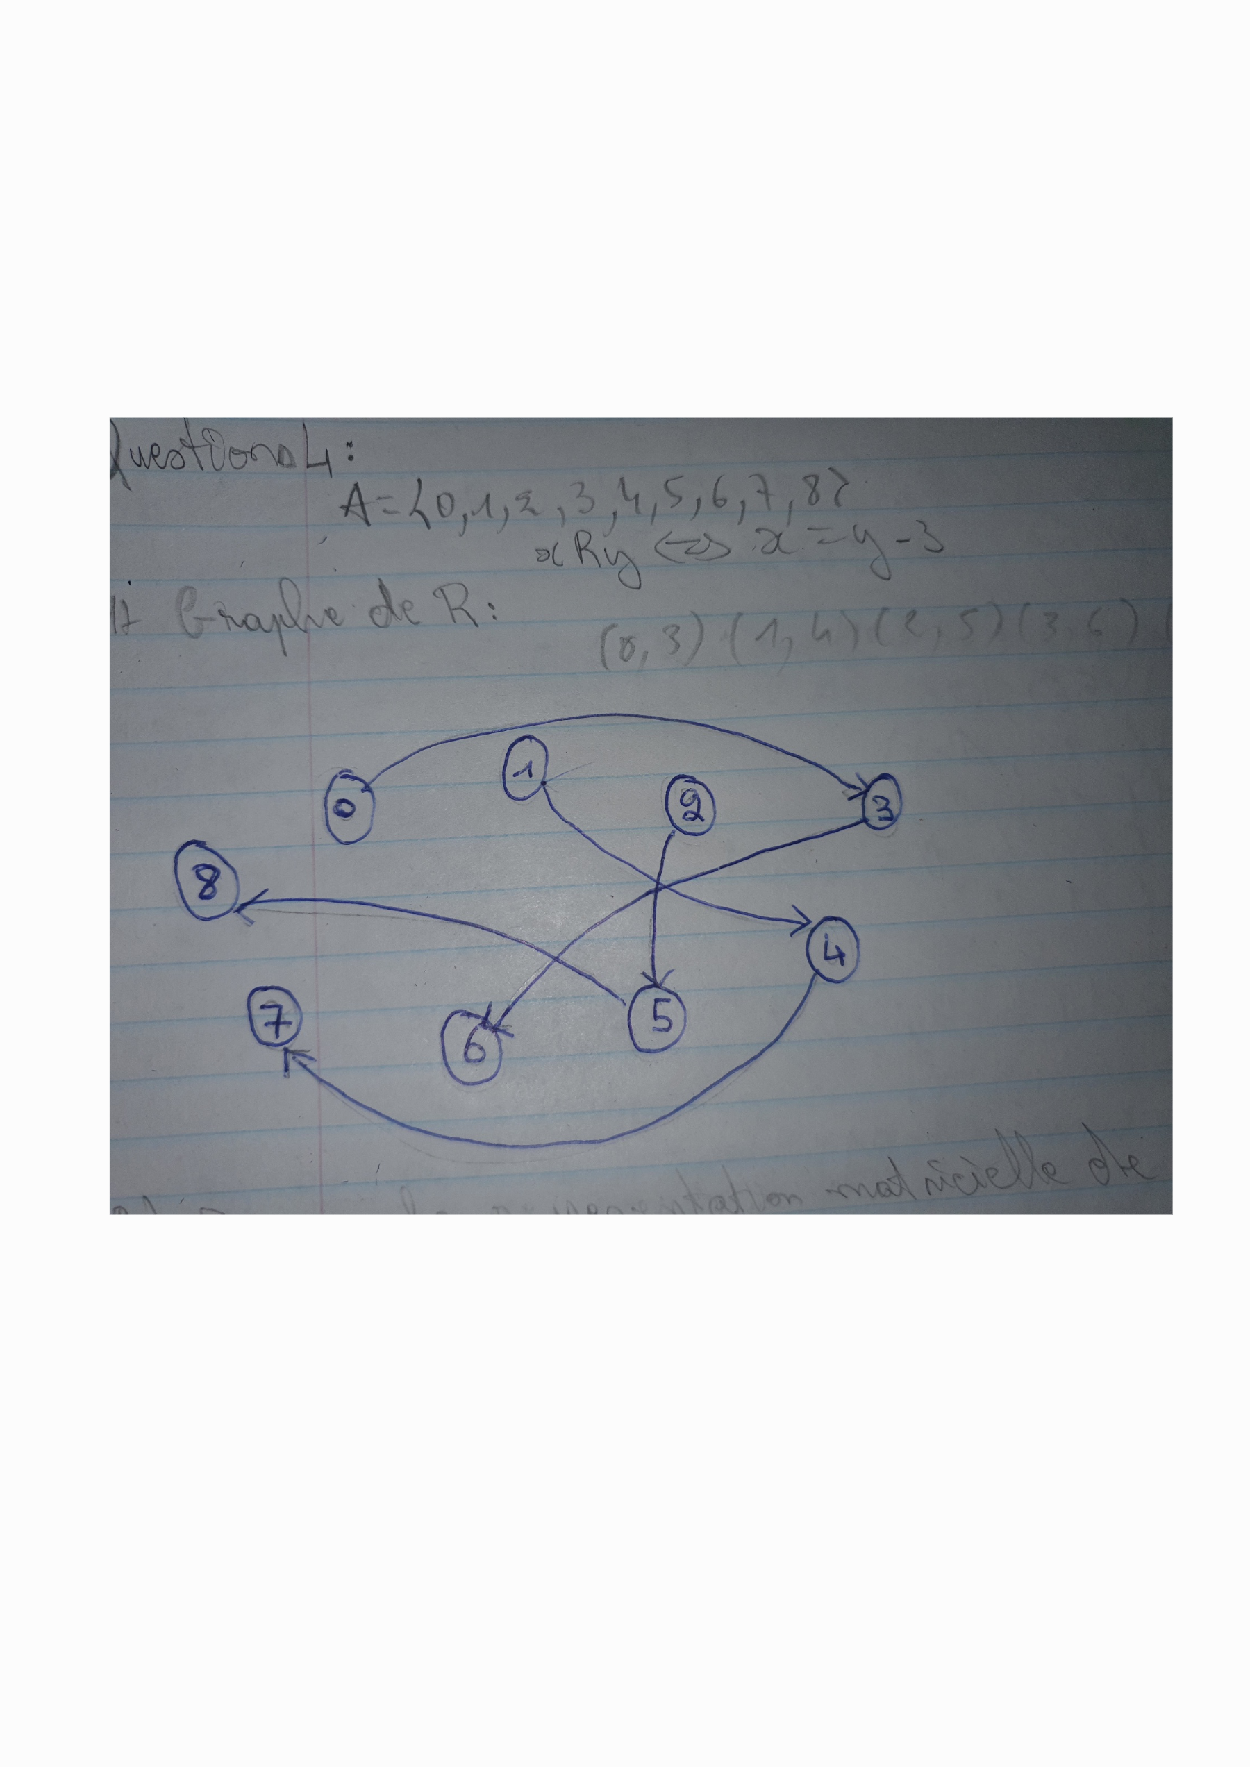
\includegraphics[width=3.5 in]{Figures/Graphe1.pdf} 
\end{center}
\vspace{-.75cm}
\end{framed}
%%%%%%%%%%%%%%%%%%%%%%%%%%%%%%%
\item\bareme{2} Donner la représentation matricielle de $R$.
%%%%%%%%%%%%%%%%%%%%%%%%%%%%%%% 
% Solution                    %
%%%%%%%%%%%%%%%%%%%%%%%%%%%%%%%
\begin{framed}

R\'EPONSE:
 $M_R$= 
 \begin{bmatrix}
 0&0 &0&1&0&0&0&0&0\\
 0&0 &0&0&1&0&0&0&0\\
 0&0 &0&0&0&1&0&0&0\\
 0&0 &0&0&0&0&1&0&0\\
 0&0 &0&0&0&0&0&1&0\\
 0&0 &0&0&0&0&0&0&1\\
 0&0 &0&0&0&0&0&0&0\\
 0&0 &0&0&0&0&0&0&0\\
 0&0 &0&0&0&0&0&0&0\\
\end{bmatrix}

\end{framed}
%%%%%%%%%%%%%%%%%%%%%%%%%%%%%%%
\item\bareme{2} La relation $R$ est-elle réflexive? symétrique? antisymétrique? Justifiez vos réponses.
%%%%%%%%%%%%%%%%%%%%%%%%%%%%%%% 
% Solution                    %
%%%%%%%%%%%%%%%%%%%%%%%%%%%%%%%
\begin{framed}

R\'EPONSE: \\
La relation $R$ n'est pas réflexive car $x$ n'est pas en relation avec lui même. \\
La relation $R$ n'est pas symétrique car $(x,y) \in R$ mais $(y,x)$ n'appatient pas à $R$ \\
La relation $R$ est  antisymétrique car $(x,y) \in R$ mais $(y,x)$ n'appatient pas à $R$ \\
\end{framed}
%%%%%%%%%%%%%%%%%%%%%%%%%%%%%%%
\item\bareme{2} Soit $T$ la fermeture transitive de $R$. Dessiner le graphe ou donner la matrice de $T$.
%%%%%%%%%%%%%%%%%%%%%%%%%%%%%%% 
% Solution                    %
%%%%%%%%%%%%%%%%%%%%%%%%%%%%%%%
\begin{framed}

R\'EPONSE:
T la fermeture transitive de R :\\
\\
 $M_T$= 
 \begin{bmatrix}
 0&0 &0&1&0&0&1&0&0\\
 0&0 &0&0&1&0&0&1&0\\
 0&0 &0&0&0&1&0&0&1\\
 0&0 &0&0&0&0&1&0&0\\
 0&0 &0&0&0&0&0&1&0\\
 0&0 &0&0&0&0&0&0&1\\
 0&0 &0&0&0&0&0&0&0\\
 0&0 &0&0&0&0&0&0&0\\
 0&0 &0&0&0&0&0&0&0\\
\end{bmatrix}

\end{framed}
%%%%%%%%%%%%%%%%%%%%%%%%%%%%%%%
\item\bareme{2} Soit $S$ la fermeture symétrique de $R$. Dessiner le graphe ou donner la matrice de $S$.
%%%%%%%%%%%%%%%%%%%%%%%%%%%%%%% 
% Solution                    %
%%%%%%%%%%%%%%%%%%%%%%%%%%%%%%%
\begin{framed}

R\'EPONSE:
S la fermeture symétrique de R:\\
\\
$M_S$= 
 \begin{bmatrix}
 0&0 &0&1&0&0&0&0&0\\
 0&0 &0&0&1&0&0&0&0\\
 0&0 &0&0&0&1&0&0&0\\
 1&0 &0&0&0&0&1&0&0\\
 0&1 &0&0&0&0&0&1&0\\
 0&0 &1&0&0&0&0&0&1\\
 0&0 &0&1&0&0&0&0&0\\
 0&0 &0&0&1&0&0&0&0\\
 0&0 &0&0&0&1&0&0&0\\
\end{bmatrix}

\end{framed}
%%%%%%%%%%%%%%%%%%%%%%%%%%%%%%%
\item\bareme{2} Soit $U$ la fermeture symétrique de $T$. Dessiner le graphe ou donner la matrice de $U$.
$U$ est-elle transitive?
%%%%%%%%%%%%%%%%%%%%%%%%%%%%%%% 
% Solution                    %
%%%%%%%%%%%%%%%%%%%%%%%%%%%%%%%
\begin{framed}

R\'EPONSE:
 U la fermeture symétrique de T: \\
 \\
 $M_U$=
 \begin{bmatrix}
 0&0 &0&1&0&0&1&0&0\\
 0&0 &0&0&1&0&0&1&0\\
 0&0 &0&0&0&1&0&0&1\\
 1&0 &0&0&0&0&1&0&0\\
 0&1 &0&0&0&0&0&1&0\\
 0&0 &1&0&0&0&0&0&1\\
 1&0 &0&1&0&0&0&0&0\\
 0&1 &0&0&1&0&0&0&0\\
 0&0 &1&0&0&1&0&0&0\\
\end{bmatrix} \\
\\
 Cette relation n'est pas transitive car dans certains cas $(x,y)\in R$ et $(y,x)\in R$ mais $(x,x)$ n'appartient pas à $R$. \\
 Exemple: $1$ est en relation avec $7$ (1,7) et $7$ est en relation avec $1$ (7,1) mais $1$ n'est pas en relation avec $1$ (1,1).

\end{framed}
%%%%%%%%%%%%%%%%%%%%%%%%%%%%%%%

\end{enumerate}
\newpage
\textbf{Partie B} (8 points)\\

Soit $P$ la relation sur l'ensemble $\mathbb{Z}$ 
d\'efinie par
\[xPy \Longleftrightarrow x= y -  3, \] 
et $W$ la plus petite relation d'équivalence contenant $P$.
\begin{enumerate}[\bf 1.]
\item\bareme{4} Décrire les classes de $W$.
%%%%%%%%%%%%%%%%%%%%%%%%%%%%%%% 
% Solution                    %
%%%%%%%%%%%%%%%%%%%%%%%%%%%%%%%
\begin{framed}

RÉPONSE: Je decris les classes de $W$:\\
Classe 0: 0 est en relation avec 3, 3 est en reltion avec 6, 6 est en relation avec 9, ... , on constate que tous ces nombres cités sont des multiples de $3$. $W$ étant une relation d'équivalence alors en faisant la fermeture refléxive, transitive et symétrique, alors l'ensemble des multiples de 3 deviennent une classe de $W$. \\
On peut noter la relation $W$ par: $xWy \Longleftrightarrow x \equiv y \mod 3$\\
Classe 1: 1 est en relation avec 4, 4 est en reltion avec 7, 7 est en relation avec 10, ... on constate que tous ces nombres cités sont des multiples de $3$ augmentés de $1$. $W$ étant une relation d'équivalence alors en faisant la fermeture refléxive, transitive et symétrique, alors l'ensemble des multiples de 3 plus 1 deviennent une classe de $W$. \\
On peut noter la relation $W$ par: $xWy \Longleftrightarrow x \equiv y \mod 3$ \\
Classe 2:  2 est en relation avec 5, 5 est en reltion avec 8, 8 est en relation avec 11, ... on constate que tous ces nombres cités sont des multiples de $3$ diminués de $1$. $W$ étant une relation d'équivalence alors en faisant la fermeture refléxive, transitive et symétrique, alors l'ensemble des multiples de 3 moins 1 deviennent une classe de $W$. \\
On peut noter la relation $W$ par: $xWy \Longleftrightarrow x \equiv y \mod 3$ \\
\end{framed}
%%%%%%%%%%%%%%%%%%%%%%%%%%%%%%%
\item\bareme{4} Donner un représentant pour chaque classe.
%%%%%%%%%%%%%%%%%%%%%%%%%%%%%%% 
% Solution                    %
%%%%%%%%%%%%%%%%%%%%%%%%%%%%%%%
\begin{framed}

RÉPONSE:\\
Représentant de la classe 0 : [0]; \\
Représentant de la classe 1 : [1]; \\
Représentant de la classe 2 : [2]; 

\end{framed}
%%%%%%%%%%%%%%%%%%%%%%%%%%%%%%%
\item\bareme{4} (Bonus) Généraliser~:  pour toute relation $Q_n$ définie par $xQ_ny \Longleftrightarrow x= y -  n,$ décrire les classes  de la plus petite relation d'\'equivalence qui contient $Q_n$.
%%%%%%%%%%%%%%%%%%%%%%%%%%%%%%% 
% Solution                    %
%%%%%%%%%%%%%%%%%%%%%%%%%%%%%%%
\begin{framed}

RÉPONSE:\\
En général, on peut dire que toute relation $Q_n$ definie par $xQ_ny \Longleftrightarrow x = y - n$, ont $n-1$ classes de la plus petite relation d'équivalence qui contient $Q_n$. La classe d'équivalent $0$ represente l'ensemble des multiples de $n$, ensuite la classe d'equivalence $1$ represente l'ensemble des multiples de $n$ plus $2$, ainsi de suite jusqu'a la classe d'equivalence $n-1$ qui represenera l'ensemble des multiples de $n$ moins 1.

\end{framed}
%%%%%%%%%%%%%%%%%%%%%%%%%%%%%%%
\end{enumerate}

%%%%%%%%%%%%%%%%%%%%%%%
%
%   Question 4
%
%%%%%%%%%%%%%%%%%%%%%%%

{\textsc{\underline{Question 4 sur les relations  (\textbf{20} points)}}}\\

Les parties A et B sont \underline{ind\'ependantes}.\\

\textbf{Partie A} (12 points)\\

 Soit $R$ la relation sur l'ensemble $A=\{0, 1,2,3,4,5,6,7,8 \}$ d\'efinie par 
$$xRy \Longleftrightarrow x = y - 3 \quad(\mbox{on note aussi }(x,y) \in R). $$ 

\begin{enumerate}[\bf 1.]

\item\bareme{2} Dessiner le graphe de $R$.
%%%%%%%%%%%%%%%%%%%%%%%%%%%%%%% 
% Solution                    %
%%%%%%%%%%%%%%%%%%%%%%%%%%%%%%%
\begin{framed}

R\'EPONSE:
\vspace{-.75cm}
\begin{center}
    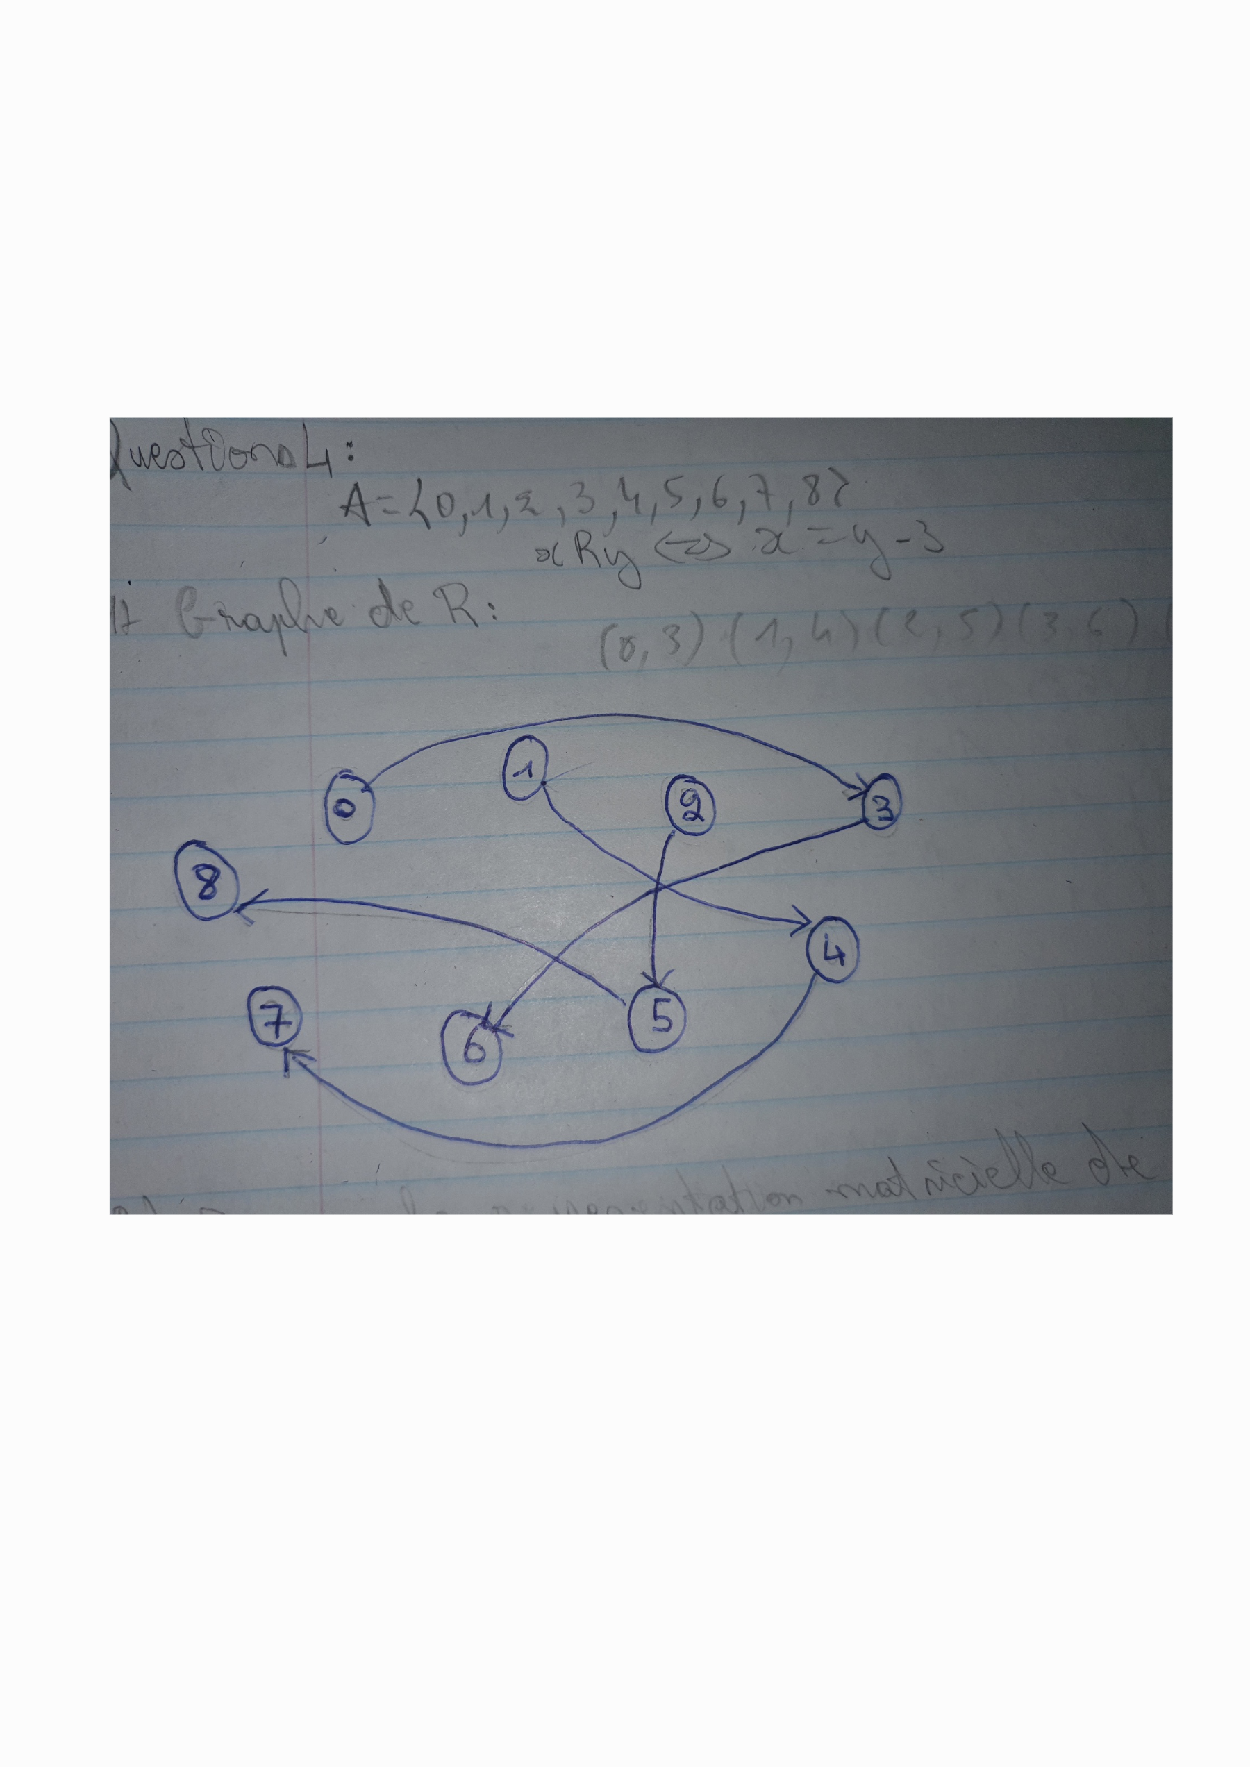
\includegraphics[width=3.5 in]{Figures/Graphe1.pdf} 
\end{center}
\vspace{-.75cm}
\end{framed}
%%%%%%%%%%%%%%%%%%%%%%%%%%%%%%%
\item\bareme{2} Donner la représentation matricielle de $R$.
%%%%%%%%%%%%%%%%%%%%%%%%%%%%%%% 
% Solution                    %
%%%%%%%%%%%%%%%%%%%%%%%%%%%%%%%
\begin{framed}

R\'EPONSE:
 $M_R$= 
 \begin{bmatrix}
 0&0 &0&1&0&0&0&0&0\\
 0&0 &0&0&1&0&0&0&0\\
 0&0 &0&0&0&1&0&0&0\\
 0&0 &0&0&0&0&1&0&0\\
 0&0 &0&0&0&0&0&1&0\\
 0&0 &0&0&0&0&0&0&1\\
 0&0 &0&0&0&0&0&0&0\\
 0&0 &0&0&0&0&0&0&0\\
 0&0 &0&0&0&0&0&0&0\\
\end{bmatrix}

\end{framed}
%%%%%%%%%%%%%%%%%%%%%%%%%%%%%%%
\item\bareme{2} La relation $R$ est-elle réflexive? symétrique? antisymétrique? Justifiez vos réponses.
%%%%%%%%%%%%%%%%%%%%%%%%%%%%%%% 
% Solution                    %
%%%%%%%%%%%%%%%%%%%%%%%%%%%%%%%
\begin{framed}

R\'EPONSE: \\
La relation $R$ n'est pas réflexive car $x$ n'est pas en relation avec lui même. \\
La relation $R$ n'est pas symétrique car $(x,y) \in R$ mais $(y,x)$ n'appatient pas à $R$ \\
La relation $R$ est  antisymétrique car $(x,y) \in R$ mais $(y,x)$ n'appatient pas à $R$ \\
\end{framed}
%%%%%%%%%%%%%%%%%%%%%%%%%%%%%%%
\item\bareme{2} Soit $T$ la fermeture transitive de $R$. Dessiner le graphe ou donner la matrice de $T$.
%%%%%%%%%%%%%%%%%%%%%%%%%%%%%%% 
% Solution                    %
%%%%%%%%%%%%%%%%%%%%%%%%%%%%%%%
\begin{framed}

R\'EPONSE:
T la fermeture transitive de R :\\
\\
 $M_T$= 
 \begin{bmatrix}
 0&0 &0&1&0&0&1&0&0\\
 0&0 &0&0&1&0&0&1&0\\
 0&0 &0&0&0&1&0&0&1\\
 0&0 &0&0&0&0&1&0&0\\
 0&0 &0&0&0&0&0&1&0\\
 0&0 &0&0&0&0&0&0&1\\
 0&0 &0&0&0&0&0&0&0\\
 0&0 &0&0&0&0&0&0&0\\
 0&0 &0&0&0&0&0&0&0\\
\end{bmatrix}

\end{framed}
%%%%%%%%%%%%%%%%%%%%%%%%%%%%%%%
\item\bareme{2} Soit $S$ la fermeture symétrique de $R$. Dessiner le graphe ou donner la matrice de $S$.
%%%%%%%%%%%%%%%%%%%%%%%%%%%%%%% 
% Solution                    %
%%%%%%%%%%%%%%%%%%%%%%%%%%%%%%%
\begin{framed}

R\'EPONSE:
S la fermeture symétrique de R:\\
\\
$M_S$= 
 \begin{bmatrix}
 0&0 &0&1&0&0&0&0&0\\
 0&0 &0&0&1&0&0&0&0\\
 0&0 &0&0&0&1&0&0&0\\
 1&0 &0&0&0&0&1&0&0\\
 0&1 &0&0&0&0&0&1&0\\
 0&0 &1&0&0&0&0&0&1\\
 0&0 &0&1&0&0&0&0&0\\
 0&0 &0&0&1&0&0&0&0\\
 0&0 &0&0&0&1&0&0&0\\
\end{bmatrix}

\end{framed}
%%%%%%%%%%%%%%%%%%%%%%%%%%%%%%%
\item\bareme{2} Soit $U$ la fermeture symétrique de $T$. Dessiner le graphe ou donner la matrice de $U$.
$U$ est-elle transitive?
%%%%%%%%%%%%%%%%%%%%%%%%%%%%%%% 
% Solution                    %
%%%%%%%%%%%%%%%%%%%%%%%%%%%%%%%
\begin{framed}

R\'EPONSE:
 U la fermeture symétrique de T: \\
 \\
 $M_U$=
 \begin{bmatrix}
 0&0 &0&1&0&0&1&0&0\\
 0&0 &0&0&1&0&0&1&0\\
 0&0 &0&0&0&1&0&0&1\\
 1&0 &0&0&0&0&1&0&0\\
 0&1 &0&0&0&0&0&1&0\\
 0&0 &1&0&0&0&0&0&1\\
 1&0 &0&1&0&0&0&0&0\\
 0&1 &0&0&1&0&0&0&0\\
 0&0 &1&0&0&1&0&0&0\\
\end{bmatrix} \\
\\
 Cette relation n'est pas transitive car dans certains cas $(x,y)\in R$ et $(y,x)\in R$ mais $(x,x)$ n'appartient pas à $R$. \\
 Exemple: $1$ est en relation avec $7$ (1,7) et $7$ est en relation avec $1$ (7,1) mais $1$ n'est pas en relation avec $1$ (1,1).

\end{framed}
%%%%%%%%%%%%%%%%%%%%%%%%%%%%%%%

\end{enumerate}
\newpage
\textbf{Partie B} (8 points)\\

Soit $P$ la relation sur l'ensemble $\mathbb{Z}$ 
d\'efinie par
\[xPy \Longleftrightarrow x= y -  3, \] 
et $W$ la plus petite relation d'équivalence contenant $P$.
\begin{enumerate}[\bf 1.]
\item\bareme{4} Décrire les classes de $W$.
%%%%%%%%%%%%%%%%%%%%%%%%%%%%%%% 
% Solution                    %
%%%%%%%%%%%%%%%%%%%%%%%%%%%%%%%
\begin{framed}

RÉPONSE: Je decris les classes de $W$:\\
Classe 0: 0 est en relation avec 3, 3 est en reltion avec 6, 6 est en relation avec 9, ... , on constate que tous ces nombres cités sont des multiples de $3$. $W$ étant une relation d'équivalence alors en faisant la fermeture refléxive, transitive et symétrique, alors l'ensemble des multiples de 3 deviennent une classe de $W$. \\
On peut noter la relation $W$ par: $xWy \Longleftrightarrow x \equiv y \mod 3$\\
Classe 1: 1 est en relation avec 4, 4 est en reltion avec 7, 7 est en relation avec 10, ... on constate que tous ces nombres cités sont des multiples de $3$ augmentés de $1$. $W$ étant une relation d'équivalence alors en faisant la fermeture refléxive, transitive et symétrique, alors l'ensemble des multiples de 3 plus 1 deviennent une classe de $W$. \\
On peut noter la relation $W$ par: $xWy \Longleftrightarrow x \equiv y \mod 3$ \\
Classe 2:  2 est en relation avec 5, 5 est en reltion avec 8, 8 est en relation avec 11, ... on constate que tous ces nombres cités sont des multiples de $3$ diminués de $1$. $W$ étant une relation d'équivalence alors en faisant la fermeture refléxive, transitive et symétrique, alors l'ensemble des multiples de 3 moins 1 deviennent une classe de $W$. \\
On peut noter la relation $W$ par: $xWy \Longleftrightarrow x \equiv y \mod 3$ \\
\end{framed}
%%%%%%%%%%%%%%%%%%%%%%%%%%%%%%%
\item\bareme{4} Donner un représentant pour chaque classe.
%%%%%%%%%%%%%%%%%%%%%%%%%%%%%%% 
% Solution                    %
%%%%%%%%%%%%%%%%%%%%%%%%%%%%%%%
\begin{framed}

RÉPONSE:\\
Représentant de la classe 0 : [0]; \\
Représentant de la classe 1 : [1]; \\
Représentant de la classe 2 : [2]; 

\end{framed}
%%%%%%%%%%%%%%%%%%%%%%%%%%%%%%%
\item\bareme{4} (Bonus) Généraliser~:  pour toute relation $Q_n$ définie par $xQ_ny \Longleftrightarrow x= y -  n,$ décrire les classes  de la plus petite relation d'\'equivalence qui contient $Q_n$.
%%%%%%%%%%%%%%%%%%%%%%%%%%%%%%% 
% Solution                    %
%%%%%%%%%%%%%%%%%%%%%%%%%%%%%%%
\begin{framed}

RÉPONSE:\\
En général, on peut dire que toute relation $Q_n$ definie par $xQ_ny \Longleftrightarrow x = y - n$, ont $n-1$ classes de la plus petite relation d'équivalence qui contient $Q_n$. La classe d'équivalent $0$ represente l'ensemble des multiples de $n$, ensuite la classe d'equivalence $1$ represente l'ensemble des multiples de $n$ plus $2$, ainsi de suite jusqu'a la classe d'equivalence $n-1$ qui represenera l'ensemble des multiples de $n$ moins 1.

\end{framed}
%%%%%%%%%%%%%%%%%%%%%%%%%%%%%%%
\end{enumerate}


\newpage

%%%%%%%%%%%%%%%%%%%%%%%
%
%   Question 5
%
%%%%%%%%%%%%%%%%%%%%%%%

%\input{devoirs/A2022/D2_A2022/Q5_graphes}
\input{Q5_graphes}

\end{document}